\documentclass{beamer}
\usepackage{../../shared/styles/custom}
\usepackage{../../shared/styles/conventions}
\usepackage{comment}

\usepackage{multicol}
%\beamerdefaultoverlayspecification{<+->}

\makeatletter
\def\magicomadjust{0em}  % a way to adjust if the spacing should be different
\newdimen\indent@amount
\def\magicom{\relax
  \ifhmode $$%
    \predisplaypenalty\@M \postdisplaypenalty\@M
    \abovedisplayskip-\baselineskip \belowdisplayskip\z@
    \abovedisplayshortskip\abovedisplayskip
    \belowdisplayshortskip\belowdisplayskip
    \global\indent@amount\predisplaysize
     $$\count@\prevgraf \advance\count@-\thr@@
         \prevgraf\count@
    \global\advance\indent@amount-2em  % correction for \predisplaysize indent
    \global\advance\indent@amount\magicomadjust  % correction for verse env, for example
    \hspace*\indent@amount
  \else\typeout{*Not in hmode*}\fi}
\makeatother

\begin{comment}

	\ifx\relax#1\relax  \item \else \item[#1] \fi
	\abovedisplayskip=0pt\abovedisplayshortskip=0pt~\vspace*{-\baselineskip}}

\end{comment}

\title{Support Vector Machines}
\date{\today}
\author{Nipun Batra}
\institute{IIT Gandhinagar}

\begin{document}
\maketitle

\begin{frame}For a point $\vx_1$ on plane 1 and $\vx_2$ on plane 2, we have:
\pause $$
\begin{array}{l}
{\vx_{2}=\vx_{1}+t \vw} \\
{D=|t \vw|=|t|\|\vw\|}
\end{array}
$$

\pause We can rewrite as follows:
\pause $$
\begin{array}{c}
{\vw \cdot \vx_{2}+b_{2}=0} \\
{\Rightarrow \vw \cdot\left(\vx_{1}+t \vw\right)+b_{2}=0}
\end{array}
$$
\pause $$
\Rightarrow \vw \cdot \vx_{1}+t\|\vw\|^{2}+b_1-b_1+b_2 = 0
\Rightarrow t = \frac{b_1 - b_2}{\|\vw\|^{2}}  \Rightarrow D = t\|\vw\| =  \frac{|b_1 - b_2|}{\|\vw\|}
$$
\end{frame}

\begin{frame}\textbf{Answer:} $D = \frac{|3 - (-1)|}{2} = \frac{4}{2} = 2$ units

\end{popquizbox}
\end{frame}

\section{SVM Formulation}

{
	\setbeamercolor{background canvas}{bg=}
	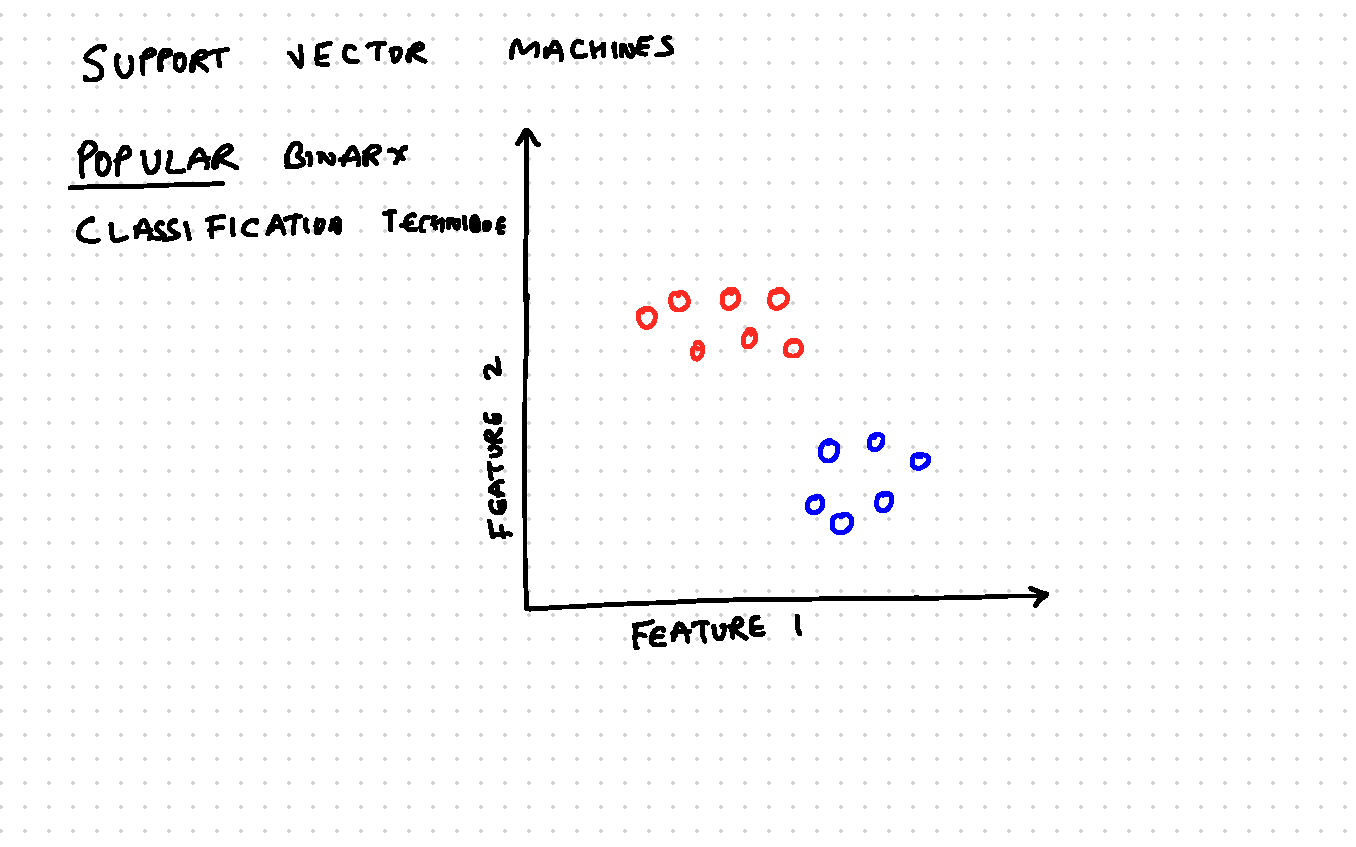
\includepdf[page=20-25]{../assets/svm/Svm-notes.pdf}
}

\begin{frame}Q) What is $\norm{\vw}$?
\pause
\begin{multicols}{2}
\begin{equation*}
	 \vw = \begin{bmatrix}
	 w_{1} \\
     w_{2} \\
     \vdots  \\
     w_{n} \\
	\end{bmatrix}
\end{equation*}\break
\begin{align*}
	 \norm{\vw} &= \sqrt{\vw\tp\vw}\\
	 &= \sqrt{\begin{bmatrix}
	 w_{1} & w_{2} & \cdots & w_{n}
	 \end{bmatrix}
	 \begin{bmatrix}
	  w_{1} \\
	  w_{2} \\
     \vdots  \\
     w_{n} \\
	 \end{bmatrix}}
\end{align*}

\end{multicols}

\end{frame}

\section{Worked Example}

{
	\setbeamercolor{background canvas}{bg=}
	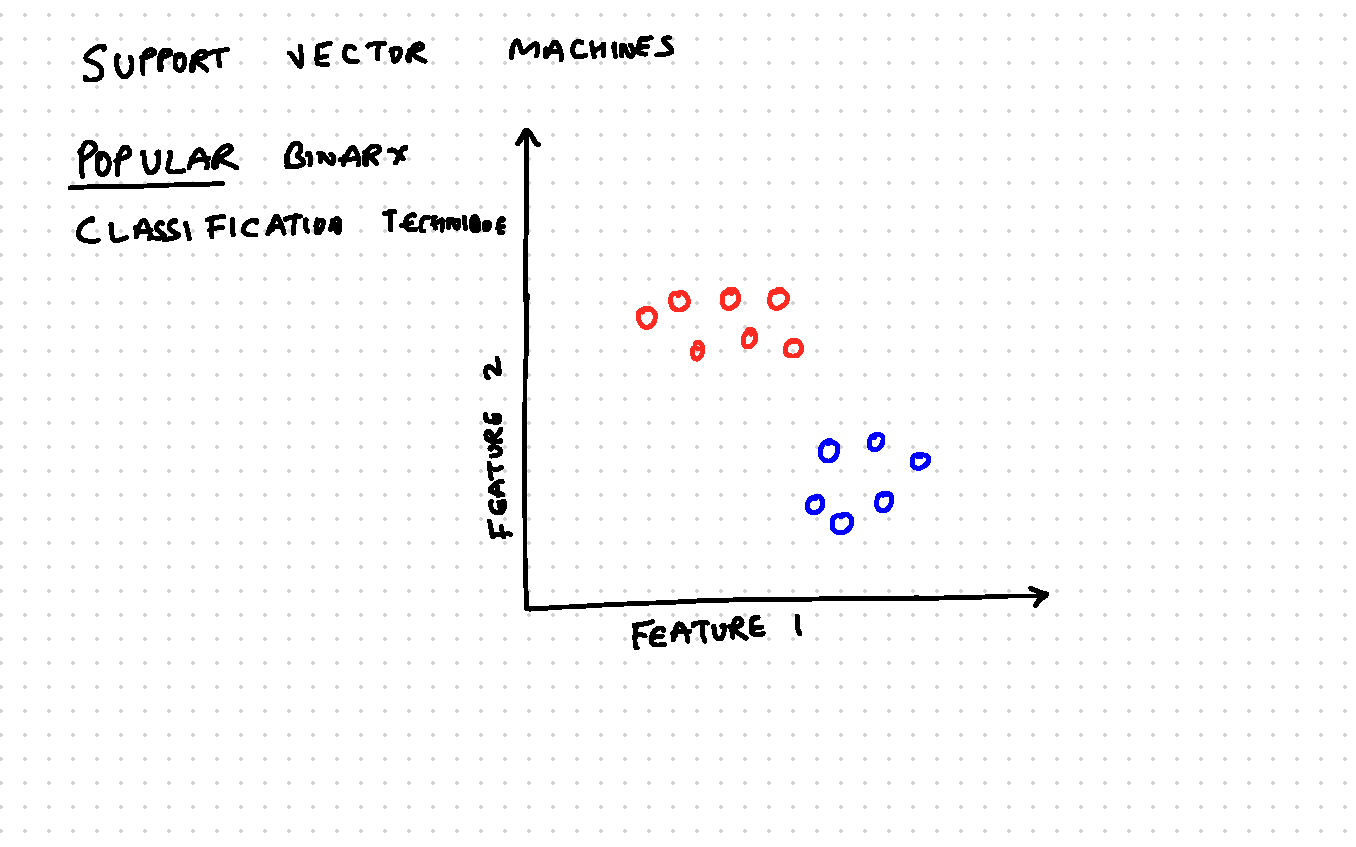
\includepdf[page=27]{../assets/svm/Svm-notes.pdf}
}

\begin{frame}\begin{itemize}
\item Is this the \textbf{only} solution that separates the data?
	\pause
\item What makes this solution \textbf{optimal} for SVM?
\end{itemize}

\pause
\textbf{Answer:} No, infinitely many solutions exist (e.g., $w = 2, b = 0$ or $w = 0.5, b = 0$). \\
SVM chooses $w = 1, b = 0$ because it minimizes $\|\vw\|^2$ while satisfying all constraints!
\end{tcolorbox}
\end{frame}

\begin{frame}\textbf{Hint:} Think about what the dual formulation enables us to do that the primal doesn't...

\pause
\textbf{Answer:} The dual formulation enables the \textbf{kernel trick}! 
\begin{itemize}
\item Primal: $\vw$ appears explicitly $\rightarrow$ no kernels
	\item Dual: Only dot products $\vx_i \cdot \vx_j$ appear $\rightarrow$ can replace with $K(\vx_i, \vx_j)$
\end{itemize}
\end{tcolorbox}
\end{frame}

\begin{frame}\textbf{Think:} Support vectors are the closest points to the decision boundary that actively constrain the solution.

\pause
\textbf{Answer:} Points $(1,+1)$ and $(-1,-1)$ are the support vectors!
\begin{itemize}
\item These are closest to the decision boundary $x = 0$
	\item They satisfy $y_i(w \cdot x_i + b) = 1$ exactly
	\pause
\item Points $(2,+1)$ and $(-2,-1)$ are farther away $\Rightarrow$ $\alpha = 0$
\end{itemize}
\end{tcolorbox}
\end{frame}

\begin{frame}\textbf{Method 1:} Direct: $\yhat(-0.5) = \sign(1 \times (-0.5) + 0) = \sign(-0.5) = -1$

\pause  
\textbf{Method 2:} Using support vectors:
$\yhat(-0.5) = \sign(\frac{1}{2} \times 1 \times 1 \times (-0.5) + \frac{1}{2} \times (-1) \times (-1) \times (-0.5))$
$ = \sign(-0.5) = -1$ (Correct!)
\end{tcolorbox}
\end{frame}

\section{Kernel Methods}

{
	\setbeamercolor{background canvas}{bg=}
	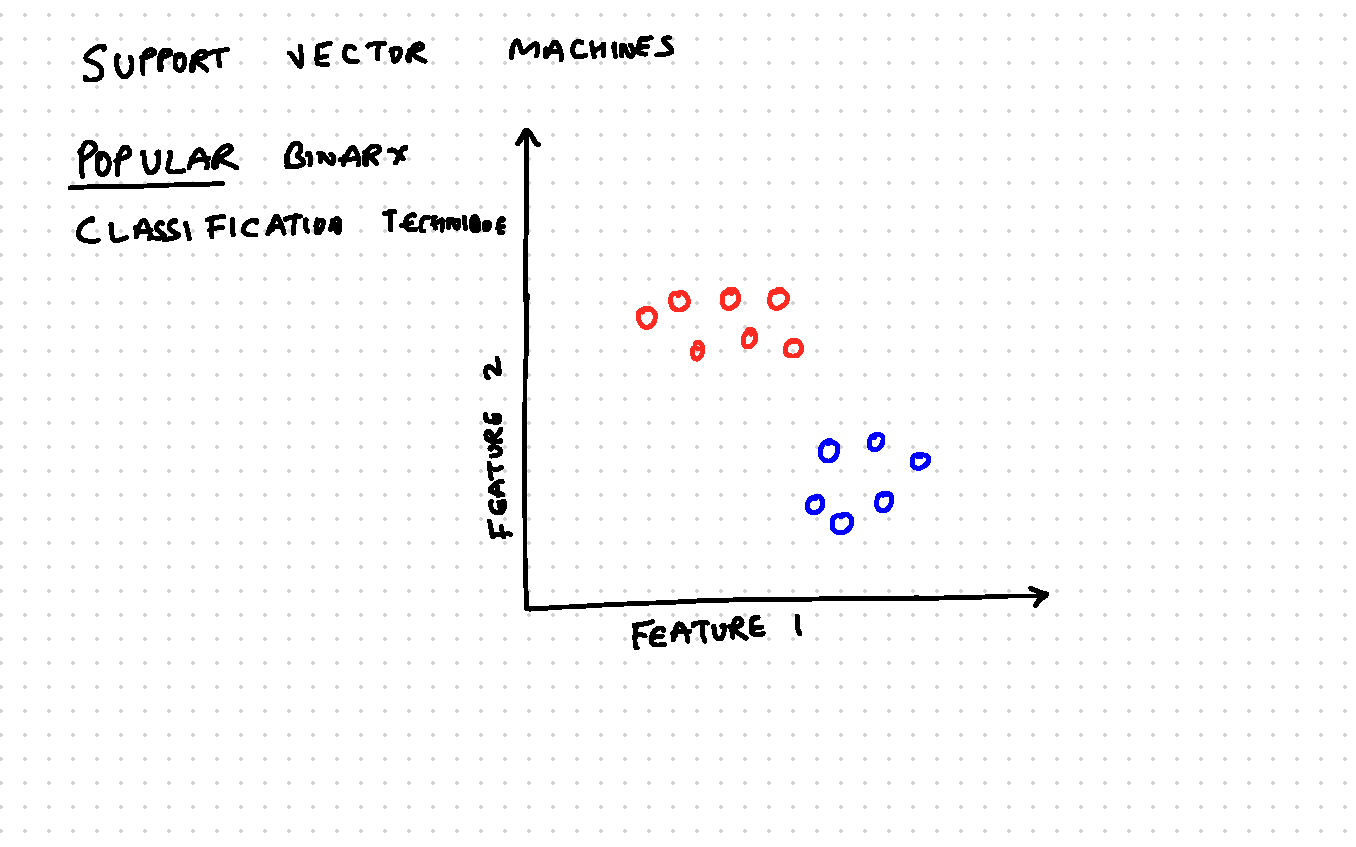
\includepdf[page=35-35]{../assets/svm/Svm-notes.pdf}
}

\begin{frame}\textbf{Expanding the squared term:}
	$$(x - z)^{2} = x^{2} - 2xz + z^{2}$$
	
	\pause
	\textbf{Substituting back into the RBF kernel:}
	\begin{align*}
	K(x, z) &= \exp(-\gamma(x^{2}-2xz+z^{2})) \\
	&= \exp(-\gamma x^{2}) \cdot \exp(2\gamma xz) \cdot \exp(-\gamma z^{2})
	\end{align*}
	
	\textbf{Key insight:} The middle term $\exp(2\gamma xz)$ contains the dot product $xz$ from the original space!
	\end{frame}
	
	\begin{frame}\textbf{Answer:} It depends on the kernel!
	    
	    \begin{itemize}
\item \textbf{Parametric:} Linear and polynomial kernels
	    		\begin{itemize}
	    			\item Fixed functional form
	    			\pause
\item Number of parameters independent of training data size
	    		\end{itemize}
	    	\item \textbf{Non-parametric:} RBF kernel
	    		\begin{itemize}
\item Model complexity grows with data
	    			\item Uses all support vectors for prediction
	    		\end{itemize}
	    \end{itemize}
	\end{frame}
	\begin{frame}{RBF is Non-Parametric}
	    \begin{align*}
	        \yhat(\vx_{\text{test}}) &= \sign(\vw \cdot \vx_{\text{test}} + b) \\
	        &= \sign(\sum_{j=1}^{N_{\text{SV}}}\alpha_{j}y_{j}\vx_{j} \cdot \vx_{\text{test}} + b)\\
	        \yhat(\vx_{\text{test}}) &= \sign(\sum_{j=1}^{N}\alpha_{j}y_{j} K(\vx_{j}, \vx_{\text{test}}) + b)
	    \end{align*}
	    $\alpha_{j} = 0$ where $j \neq$ S.V.
	\end{frame}

	\begin{frame}{Interpretation of RBF}
		\begin{itemize}
\item $\yhat(\vx) = \sign(\sum \alpha_{i}y_{i}\exp(-\norm{\vx - \vx_{i}}^{2}) + b)$
			\item $-\norm{\vx - \vx_{i}}^{2}$ corresponds to radial term
			\pause
\item $\sum \alpha_{i}y_{i}$ is the activation component
			\item $\exp(-\norm{\vx - \vx_{i}}^{2})$ is the basis component
		\end{itemize}

	\end{frame}

\subsection{Kernel Properties}

		{
	\setbeamercolor{background canvas}{bg=}
	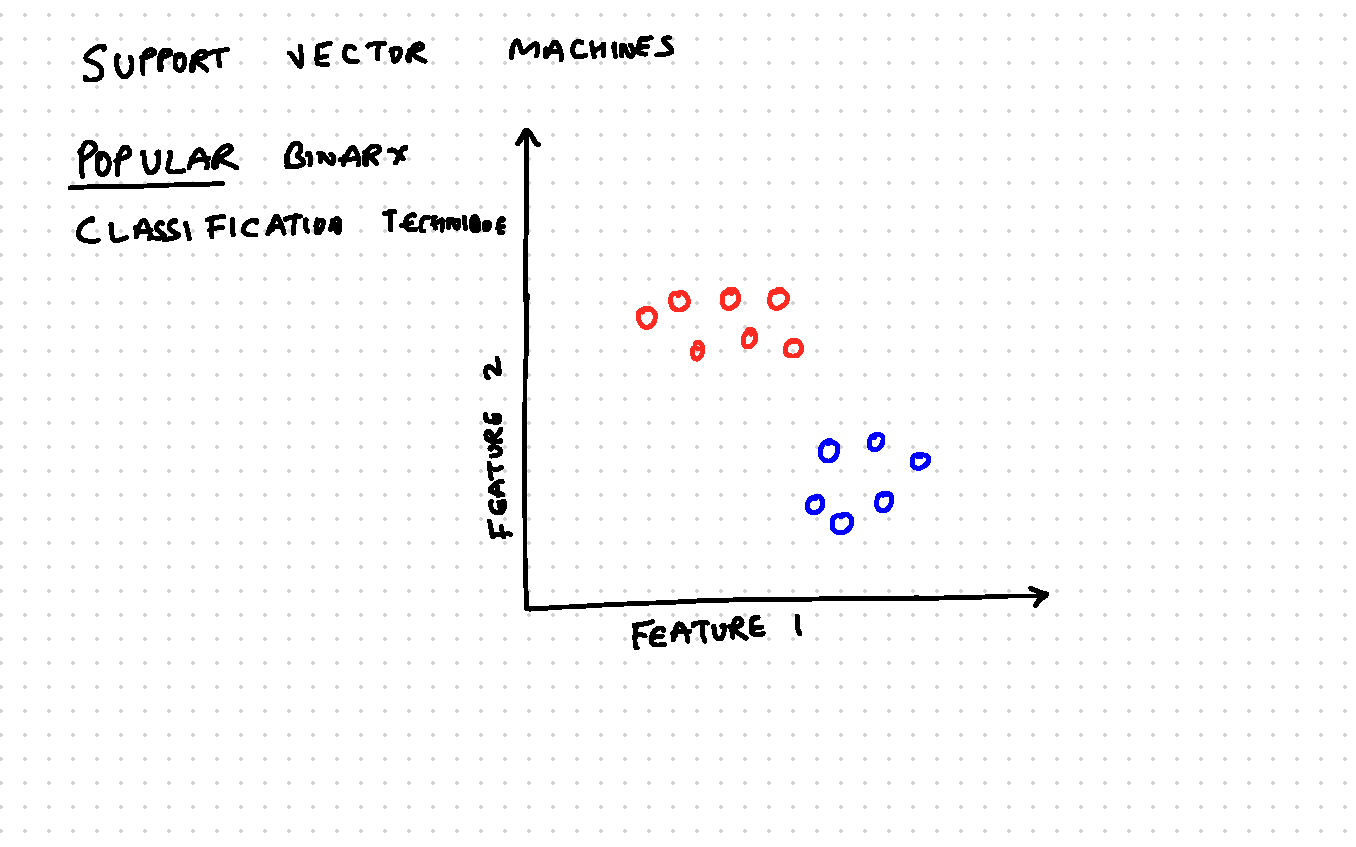
\includepdf[page=48-49]{../assets/svm/Svm-notes.pdf}
}

\section{Summary}

\begin{frame}{Key Takeaways}
\begin{itemize}
\item \textbf{Goal:} SVM finds optimal separating hyperplane by maximizing margin
	\pause
\item \textbf{Math:} Dual formulation enables kernel trick
	\pause
\item \textbf{Power:} Kernels enable non-linear classification without explicit mapping
	\pause
\item \textbf{Popular kernels:} Linear, Polynomial, RBF (Gaussian)
	\pause
\item \textbf{Remarkable:} RBF kernel $\leftrightarrow$ infinite-dimensional space
	\pause
\item \textbf{Flexibility:} Parametric (linear/poly) or non-parametric (RBF)
	\pause
\item \textbf{Efficiency:} Only support vectors matter for prediction
\end{itemize}
\end{frame}

\begin{frame}{Next Steps}
\begin{itemize}
\item Soft-margin SVM for non-separable data
	\item Hyperparameter tuning (C, $\gamma$)
	\pause
\item Multi-class SVM extensions
	\item Computational considerations and optimization
	\item Comparison with other classifiers
\end{itemize}
\end{frame}

\end{document}
